\documentclass[a4paper]{article}

% Use these
%\usepackage{times}
%\usepackage{helvet}
%\usepackage{courier}
%\usepackage{graphicx}
%\usepackage{epsfig}
\usepackage{subfigure}
%\usepackage{enumerate}
%\usepackage{pdfpages}
%\usepackage{float}
%\usepackage{xspace}

%% Use these
\usepackage{tikz}
\usetikzlibrary{arrows,decorations,backgrounds,matrix,automata,trees,shapes,shadows,plotmarks,calc}
\usepackage{pgflibraryshapes}

%% Allow page margins to be changed for specified block
\def\changemargin#1#2{\list{}{\rightmargin#2\leftmargin#1}\item[]}
\let\endchangemargin=\endlist 


%% Set fbox defaults
\setlength\fboxsep{5pt}
  
%% Begin
\title{BDI-Learning Discussion Paper \#4:\\A Complexity-based Confidence Measure}

\author{
Dhirendra Singh\\ 
dhirendra.singh@rmit.edu.au\\
}

\begin{document}

%\date{7 July 2009}

\maketitle

%%
\section{Background and Scope}

This document is a corollary of the HYCAS submission~\cite{Singh:HYCAS10} and should be read in conjunction with the same. The focus of this document is modifications to the complexity based confidence measure plus fixes for any open issues with the proposal.

%%
\section{Recent Changes}

\subsection{Complexity Calculation}

For our purposes, when we talk about \textit{complexity} of the goal-plan tree node we refer to the number of paths below that node in the structure. Where the notion of \textit{coverage}~\cite{Singh:AAMAS10} was an accurate representation of these paths, complexity is intended to be an approximation that is calculated based on certain properties of the goal-plan tree. In~\cite{Singh:HYCAS10}, however, this approximation is not computed but rather user specified for each plan in the example domain (Towers of Hanoi). 

The proposed change for complexity calculations is as follows: For non-recursive nodes use $\eta = \rho ^ \sigma$. For recursive nodes use $\eta = log_2(\delta+2) ^ {\rho ^ \sigma}$. Here $\eta$ is the complexity, $\rho$ is the maximum number of possible plan options per goal in factor for plans in the hierarchy, $\sigma$ is the maximum branching factor for goals in the hierarchy, and $\delta$ is the recursive depth.

Dhirendra to self: This should instead be a single formula for 'leaf' and  'non-leaf' (recursive or otherwise) nodes instead.

\subsection{Optimised Recording}

In an attempt to reduce the number of saved experiences over time and improve decision tree induction times we performed two optimisations. Firstly, decision tree induction is performed only when at least $k$ new experiences have been recorded. In~\cite{Singh:HYCAS10} we used $k=25$ that gives significant improvements in running times with negligible impact on overall performance. Secondly, we reduce the total number of samples used, by compacting all duplicate experiences into a single experience that uses a \textit{weight} proportional to the number of duplicates. So for a given plan then, a maximum of two instances per world are possible, one for success and one for failure, each with different individual weights.

\subsection{Confidence Calculation}

Saved experiences are used to estimate decision tree classification confidence as follows:

In~\cite{Singh:HYCAS10}, if a plan has experienced at least one success in a given world then that plan temporarily gets full confidence for that world regardless of the number of failures (the reasoning being that if a plan has succeeded in a world then there is no need to consider previous failures in the decision making). A related limitation however, is that if a successful plan starts failing (due to environmental changes for instance) then this change will go unnoticed because we disregard all failures for a previously successful plan. The fix is to reset failure counts for a given plan in a given world each time a success is experienced, and start counting failures afresh. Confidence for such previously successful worlds is then the ratio $success/attempts$.

For worlds where the plan has never been successful, confidence in the decision tree classification is a gradually increasing value based on the decay function described in~\cite{Singh:HYCAS10} (the decay is faster for small sub-trees and slower for more complex ones).

One important issue with the decay-based confidence calculation is that it does not consider the point of failure. So, for instance, a very complex plan structure that fails at the root will still be tried numerous times since the decision tree confidence increases very slowly for such a complex hierarchy. The solution is to adjust the decay based on not only the complexity of the plan sub-tree but also on the complexity of the sub-tree at the point of failure. Previously, the decay was calculated as $\delta = \delta * [1 - (1/\eta_p)]$ where $\eta_p$ is the complexity of the calculating node. The modification means that the decay is now calculated as $\delta = \delta * [1 - (1/(\eta_p-\eta_o)]$ where $\eta_o$ is the complexity of the plan at the point of failure. Intuitively, this means that the decay is faster (i.e. confidence grows more quickly) the higher up the complex sub-tree the failure occurs.

\begin{figure*}[t]
\begin{center}
\subfigure[$ACL$ with solutions at recursion levels one (pluses), three (circles) and five (crosses).]{\label{fig:result-levelsA}
\resizebox{.42\textwidth}{!}{%!TEX root = ../hycas2010.tex
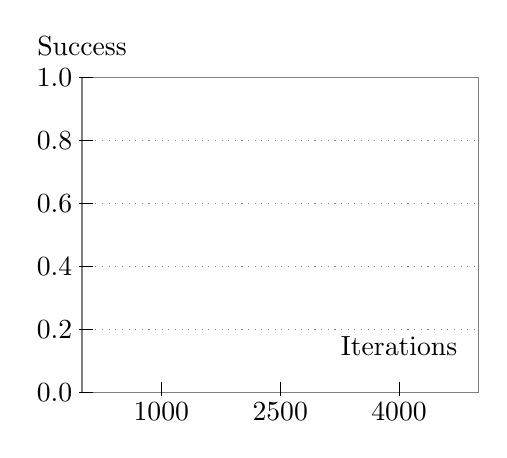
\begin{tikzpicture}[x=0.001cm,y=4cm]
    % Draw the axes and grid lines
    \draw[-,gray] (0,0) -- (0,1) -- (5000,1) -- (5000,0) -- cycle; 
    \draw[-,gray,thin, dotted, ystep=0.2, xstep=5000] (0,0) grid (5000,1);
    \foreach \x in {1000, 2500, 4000}  \draw [-,xshift=0](\x,4pt) -- (\x,-1pt);
    \foreach \y in {0.0,0.2,0.4,0.6,0.8,1.0}  \draw [-,yshift=0](4pt,\y) -- (-1pt,\y);
    \foreach \x/\xtext in {1000/1000, 2500/2500, 4000/4000} \node at (\x,0) [below] {$\xtext$};
    \foreach \y/\ytext in {0.0,0.2,0.4,0.6,0.8,1.0}  \node at (0,\y) [left] {$\ytext$};
    \node at (0,1.1) {Success};
    \node at (4000,0.15) {Iterations};
    \draw[-,gray] plot[mark=+,mark size=4,mark options={color=black}] 
			file {data/hanoid5s1r8.CP.tikzdata};
    \draw[-,gray] plot[mark=o,mark size=3,mark options={color=black}] 
			file {data/hanoid5s3r8.CP.tikzdata};
    \draw[-,gray] plot[mark=x,mark size=4,mark options={color=black}] 
			file {data/hanoid5s5r8.CP.tikzdata};

\end{tikzpicture}
}
}
\qquad
\subfigure[$ACL+\Omega$ with solutions at recursion levels one (pluses), three (circles) and five (crosses).]{\label{fig:result-levelsB}
\resizebox{.42\textwidth}{!}{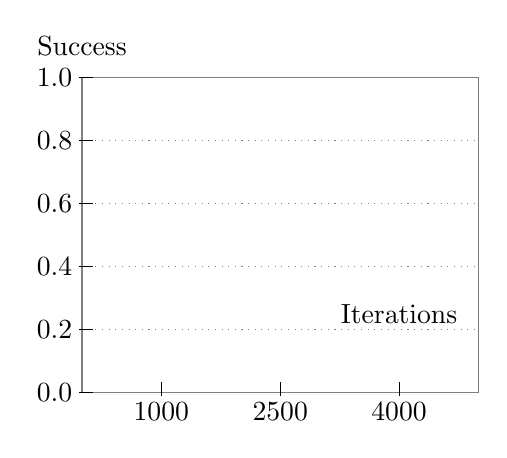
\begin{tikzpicture}[x=0.001cm,y=4cm]
    % Draw the axes and grid lines
    \draw[-,gray] (0,0) -- (0,1) -- (5000,1) -- (5000,0) -- cycle; 
    \draw[-,gray,thin, dotted, ystep=0.2, xstep=5000] (0,0) grid (5000,1);
    \foreach \x in {1000, 2500, 4000}  \draw [-,xshift=0](\x,4pt) -- (\x,-1pt);
    \foreach \y in {0.0,0.2,0.4,0.6,0.8,1.0}  \draw [-,yshift=0](4pt,\y) -- (-1pt,\y);
    \foreach \x/\xtext in {1000/1000, 2500/2500, 4000/4000} \node at (\x,0) [below] {$\xtext$};
    \foreach \y/\ytext in {0.0,0.2,0.4,0.6,0.8,1.0}  \node at (0,\y) [left] {$\ytext$};
    \node at (0,1.1) {Success};
    \node at (4000,0.25) {Iterations};
    \draw[-,gray] plot[mark=+,mark size=4,mark options={color=black}] 
			file {data/hanoid5s1r8.CF.tikzdata};
    \draw[-,gray] plot[mark=o,mark size=3,mark options={color=black}] 
			file {data/hanoid5s3r8.CF.tikzdata};
    \draw[-,gray] plot[mark=x,mark size=4,mark options={color=black}] 
			file {data/hanoid5s5r8.CF.tikzdata};

\end{tikzpicture}
}
}
\qquad
\subfigure[$ACL$ (circles) and $ACL+\Omega$ (crosses) schemes with applicability threshold $0\%$]{\label{fig:result-fullA}
\resizebox{.42\textwidth}{!}{../../../writeup/2010HYCAS/figs/result-fullA.tex}
}
\qquad
\subfigure[$ACL$ (circles) and $ACL+\Omega$ (crosses) schemes with applicability threshold $20\%$]{\label{fig:result-fullB}
\resizebox{.42\textwidth}{!}{%!TEX root = ../hycas2010.tex
% Points in the input file are x-scaled by 0.5 so xval 1000 represents point 2000 in the original results. The reason for scaling was that TeX cannot handle > ~16k numbers
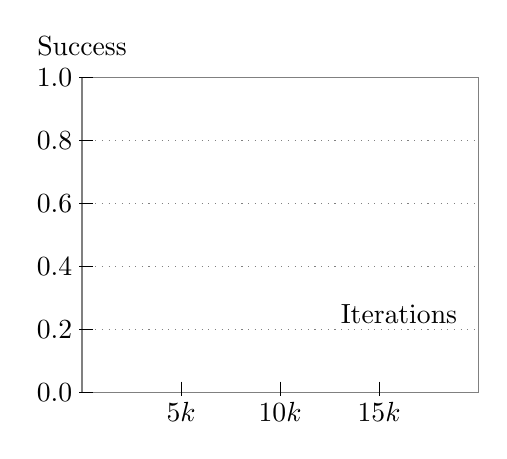
\begin{tikzpicture}[x=0.0005cm,y=4cm]
    % Draw the axes and grid lines
    \draw[-,gray] (0,0) -- (0,1) -- (10000,1) -- (10000,0) -- cycle; 
    \draw[-,gray,thin, dotted, ystep=0.2, xstep=10000] (0,0) grid (10000,1);
    \foreach \x in {2500, 5000, 7500}  \draw [-,xshift=0](\x,4pt) -- (\x,-1pt);
    \foreach \y in {0.0,0.2,0.4,0.6,0.8,1.0}  \draw [-,yshift=0](4pt,\y) -- (-1pt,\y);
    \foreach \x/\xtext in {2500/5k, 5000/10k, 7500/15k} \node at (\x,0) [below] {$\xtext$};
    \foreach \y/\ytext in {0.0,0.2,0.4,0.6,0.8,1.0}  \node at (0,\y) [left] {$\ytext$};
    \node at (0,1.1) {Success};
    \node at (8000,0.25) {Iterations};
    \draw[-,gray] plot[mark=o,mark size=3,mark options={color=black}] 
			file {data/hanoi5t.CP.tikzdata};
    \draw[-,gray] plot[mark=x,mark size=4,mark options={color=black}] 
			file {data/hanoi5t.CF.tikzdata};
\end{tikzpicture}
}
}
\caption{Agent performance under $ACL$ and $ACL+\Omega$ schemes. Each point represents results from $5$ experiment runs using an averaging window of $100$ samples. Reproduced from \cite{Singh:HYCAS10}.}
\label{fig:results-hycas}
\end{center}
\end{figure*}


\subsection{Accuracy Improvements}


Figure~\ref{fig:results-hycas} shows the results reproduced from \cite{Singh:HYCAS10}. There are two reasons why the $ACL+\Omega$ performance of Figure~\ref{fig:result-fullA} does not converge to $1.0$. The first reason is what was indicated in~\cite{Singh:HYCAS10} --- that the way a sub-goal is resolved may influence the parent failing or succeeding. This is because a sub-optimal resolution may increase the recursion level beyond what is legally allowed (user specified bounded recursion limit). The second reason is that decision tree classification is not always perfect even for previously successful worlds. To improve this, the following options are now passed to the $J48$ algorithm: $-C~0.5 -M~1$. See weka $J48$ documentation for details.


\subsection{Testing}

The individual recursive level tests reported in Figure~\ref{fig:result-levelsA} and Figure~\ref{fig:result-levelsB} and the full test reported in Figure~\ref{fig:result-fullA} and Figure~\ref{fig:result-fullB} are reproduced from \cite{Singh:HYCAS10} and use a \textit{subset} of all possible goal/setup configurations for each experiment. This has now been extended to include \textit{all} possible goal/setup configurations per recursive level.

\section{Results}

The final results after all the listed changes are shown in Figure~\ref{fig:results-new}. The repository revision for the final changes is $svn:323$.
\begin{figure*}[t]
\begin{center}
\subfigure[$ACL$ with solutions at recursion levels one (pluses), three (circles) and five (crosses).]{\label{fig:result-levelsAnew}
\resizebox{.42\textwidth}{!}{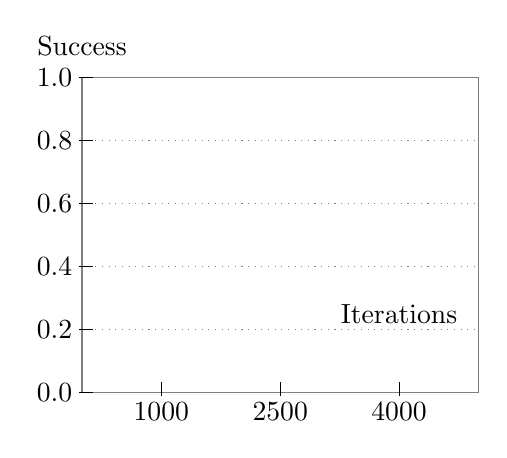
\begin{tikzpicture}[x=0.001cm,y=4cm]
    % Draw the axes and grid lines
    \draw[-,gray] (0,0) -- (0,1) -- (5000,1) -- (5000,0) -- cycle; 
    \draw[-,gray,thin, dotted, ystep=0.2, xstep=5000] (0,0) grid (5000,1);
    \foreach \x in {1000, 2500, 4000}  \draw [-,xshift=0](\x,4pt) -- (\x,-1pt);
    \foreach \y in {0.0,0.2,0.4,0.6,0.8,1.0}  \draw [-,yshift=0](4pt,\y) -- (-1pt,\y);
    \foreach \x/\xtext in {1000/1000, 2500/2500, 4000/4000} \node at (\x,0) [below] {$\xtext$};
    \foreach \y/\ytext in {0.0,0.2,0.4,0.6,0.8,1.0}  \node at (0,\y) [left] {$\ytext$};
    \node at (0,1.1) {Success};
    \node at (4000,0.25) {Iterations};
    \draw[-,gray] plot[mark=+,mark size=4,mark options={color=black}] 
			file {data/hanoid5s1r8new.CP.tikzdata};
    \draw[-,gray] plot[mark=o,mark size=3,mark options={color=black}] 
			file {data/hanoid5s3r8new.CP.tikzdata};
    \draw[-,gray] plot[mark=x,mark size=4,mark options={color=black}] 
			file {data/hanoid5s5r8new.CP.tikzdata};

\end{tikzpicture}
}
}
\qquad
\subfigure[$ACL+\Omega$ with solutions at recursion levels one (pluses), three (circles) and five (crosses).]{\label{fig:result-levelsBnew}
\resizebox{.42\textwidth}{!}{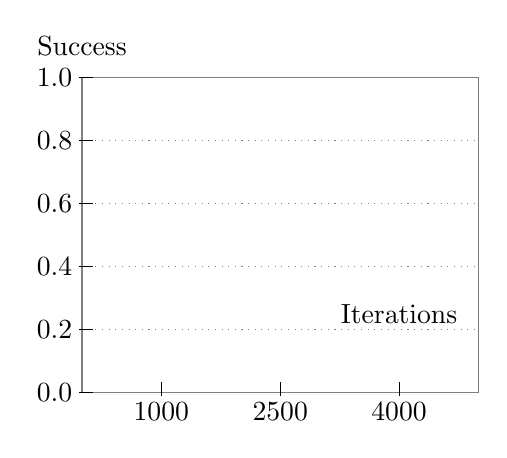
\begin{tikzpicture}[x=0.001cm,y=4cm]
    % Draw the axes and grid lines
    \draw[-,gray] (0,0) -- (0,1) -- (5000,1) -- (5000,0) -- cycle; 
    \draw[-,gray,thin, dotted, ystep=0.2, xstep=5000] (0,0) grid (5000,1);
    \foreach \x in {1000, 2500, 4000}  \draw [-,xshift=0](\x,4pt) -- (\x,-1pt);
    \foreach \y in {0.0,0.2,0.4,0.6,0.8,1.0}  \draw [-,yshift=0](4pt,\y) -- (-1pt,\y);
    \foreach \x/\xtext in {1000/1000, 2500/2500, 4000/4000} \node at (\x,0) [below] {$\xtext$};
    \foreach \y/\ytext in {0.0,0.2,0.4,0.6,0.8,1.0}  \node at (0,\y) [left] {$\ytext$};
    \node at (0,1.1) {Success};
    \node at (4000,0.25) {Iterations};
    \draw[-,gray] plot[mark=+,mark size=4,mark options={color=black}] 
			file {data/hanoid5s1r8new.CF.tikzdata};
    \draw[-,gray] plot[mark=o,mark size=3,mark options={color=black}] 
			file {data/hanoid5s3r8new.CF.tikzdata};
    \draw[-,gray] plot[mark=x,mark size=4,mark options={color=black}] 
			file {data/hanoid5s5r8new.CF.tikzdata};

\end{tikzpicture}
}
}
\qquad
\subfigure[$ACL$ (circles) and $ACL+\Omega$ (crosses) schemes with applicability threshold $0\%$]{\label{fig:result-fullAnew}
\resizebox{.42\textwidth}{!}{% Points in the input file are x-scaled by 0.5 so xval 1000 represents point 2000 in the original results. The reason for scaling was that TeX cannot handle > ~16k numbers
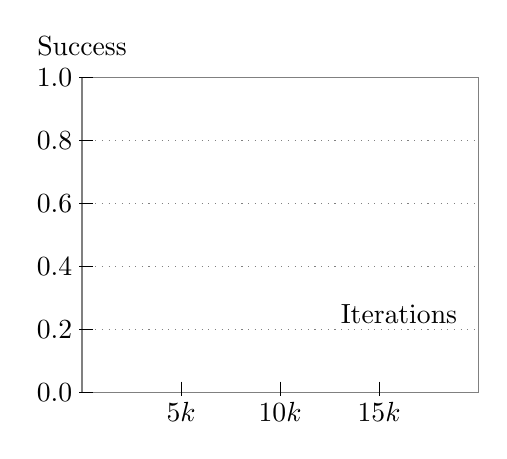
\begin{tikzpicture}[x=0.0005cm,y=4cm]
    % Draw the axes and grid lines
    \draw[-,gray] (0,0) -- (0,1) -- (10000,1) -- (10000,0) -- cycle; 
    \draw[-,gray,thin, dotted, ystep=0.2, xstep=10000] (0,0) grid (10000,1);
    \foreach \x in {2500, 5000, 7500}  \draw [-,xshift=0](\x,4pt) -- (\x,-1pt);
    \foreach \y in {0.0,0.2,0.4,0.6,0.8,1.0}  \draw [-,yshift=0](4pt,\y) -- (-1pt,\y);
    \foreach \x/\xtext in {2500/5k, 5000/10k, 7500/15k} \node at (\x,0) [below] {$\xtext$};
    \foreach \y/\ytext in {0.0,0.2,0.4,0.6,0.8,1.0}  \node at (0,\y) [left] {$\ytext$};
    \node at (0,1.1) {Success};
    \node at (8000,0.25) {Iterations};
    \draw[-,gray] plot[mark=o,mark size=3,mark options={color=black}] 
			file {data/hanoi5new.CP.tikzdata};
    \draw[-,gray] plot[mark=x,mark size=4,mark options={color=black}] 
			file {data/hanoi5new.CF.tikzdata};
\end{tikzpicture}
}
}
\qquad
\subfigure[$ACL$ (circles) and $ACL+\Omega$ (crosses) schemes with applicability threshold $20\%$]{\label{fig:result-fullBnew}
\resizebox{.42\textwidth}{!}{% Points in the input file are x-scaled by 0.5 so xval 1000 represents point 2000 in the original results. The reason for scaling was that TeX cannot handle > ~16k numbers
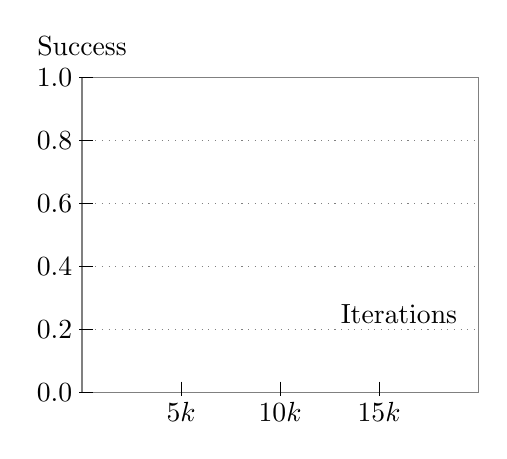
\begin{tikzpicture}[x=0.0005cm,y=4cm]
    % Draw the axes and grid lines
    \draw[-,gray] (0,0) -- (0,1) -- (10000,1) -- (10000,0) -- cycle; 
    \draw[-,gray,thin, dotted, ystep=0.2, xstep=10000] (0,0) grid (10000,1);
    \foreach \x in {2500, 5000, 7500}  \draw [-,xshift=0](\x,4pt) -- (\x,-1pt);
    \foreach \y in {0.0,0.2,0.4,0.6,0.8,1.0}  \draw [-,yshift=0](4pt,\y) -- (-1pt,\y);
    \foreach \x/\xtext in {2500/5k, 5000/10k, 7500/15k} \node at (\x,0) [below] {$\xtext$};
    \foreach \y/\ytext in {0.0,0.2,0.4,0.6,0.8,1.0}  \node at (0,\y) [left] {$\ytext$};
    \node at (0,1.1) {Success};
    \node at (8000,0.25) {Iterations};
    \draw[-,gray] plot[mark=o,mark size=3,mark options={color=black}] 
			file {data/hanoi5tnew.CP.tikzdata};
    \draw[-,gray] plot[mark=x,mark size=4,mark options={color=black}] 
			file {data/hanoi5tnew.CF.tikzdata};
\end{tikzpicture}
}
}
\caption{Agent performance under $ACL$ and $ACL+\Omega$ schemes. Each point represents results from $5$ experiment runs using an averaging window of $100$ samples. Repository revision $323$.}
\label{fig:results-new}
\end{center}
\end{figure*}

\subsection{Limitations}
Two known limitations in the treatment of recursive goals are:
\begin{itemize}
\item Only one recursive goal-type $G$ is supported in the code. This is sufficient for the simple Towers of Hanoi problem of~\cite{Singh:HYCAS10} but will have to be extended for domains where multiple recursive goal-types are possible.
\item Only $G \to P \to G$ recursion is supported where a plan posts the same goal that it handles. More complex interactions such as $G_1 \to P_1 \to G_2 \to P_2 \to G_1$ require global knowledge of goals in the system at the plan level that we do not support currently.
\end{itemize}



%%
\begin{thebibliography}{10}

\bibitem{Singh:HYCAS10}
D.~Singh, S.~Sardina, L.~Padgham.
\newblock Extending BDI Plan Selection to Incorporate Learning from Experience.
\newblock Submission under review for the Special Issue on Hybrid Control of Autonomous Systems (HYCAS), Journal of Robotics and Autonomous Systems, 2010.

\bibitem{Singh:AAMAS10}
D.~Singh, S.~Sardina, L.~Padgham, S.~Airiau.
\newblock Learning Context Conditions for {BDI} Plan Selection.
\newblock Submission under review for Proceedings of Autonomous Agents and Multi-Agent Systems (AAMAS), 2010.

\bibitem{Airiau:IJAT09}
S.~Airiau, L.~Padgham, S.~Sardina, and S.~Sen.
\newblock Enhancing Adaptation in {BDI} Agents Using Learning Techniques.
\newblock In {\em International Journal of Agent Technologies and Systems},
2009.

\end{thebibliography}

\end{document}